In this section we conducted our experiments on a heterogeneous infrastructure like Amazon EC2~\cite{amazonEC2}, and on a homogeneous infrastructure like DAS-4 (the Distributed ASCI Supercomputer 4)~\cite{das4}. DAS-4 is the Dutch Computational Infrastructure, a six-cluster wide-area distributed system designed with research purposes. In our experiment campaign, we compared the degree of SLO enforcement (performance requirements fulfillment) and resource consumption for each one of the provisioning algorithms included in ConPaaS. 


\subsection{Testbed configuration}

As a realistic and representative scenario, we deployed MediaWiki application using ConPaaS on both infrastructures, and we ran the Wikibench tools utilizing Wikipedia workload traces.  To provide the Wikipedia services, an initial configuration was composed of 4 VMs, and 1 VM to host the Wikibench tools. The 4 VMs include a PhP service manager VM, a PhP agent VM, a web server and a http-proxy agent VM (both in the same VM), and finally a MySQL agent VM to store the English Wikipedia data, as explained in Section~\ref{wikipedia}.

Our goal is to evaluate the behavior of the provisioning algorithms, when scaling out and back the number of VMs hosting PhP servers to guarantee several performance requirements, referred to as SLO. Specifically, we fixed two SLOs, one of 700 milliseconds at the service's side (denoted by a yellow Line on Figures~\ref{naiveDas4},\ref{historyDas4},\ref{naiveEC2},\ref{historyEC2} and \ref{historyWeightEC2}), and another of 1500 milliseconds at the client's side (denoted by a red Line on Figures~\ref{naiveDas4},\ref{historyDas4},\ref{naiveEC2},\ref{historyEC2} and \ref{historyWeightEC2}). Thus, our measurements shows the behavior of the MediaWiki application under a workload generated from real access traces during 24h. Note that, these experiments only focus on the average of PhP response times and the resource consumption obtained with our algorithms. 

\noindent Accordingly, some assumptions were made:

\begin{itemize}
\item  Response times from static requests were not analyzed due to the lightweight nature of the static files employed by Wikipedia articles. 

\item The algorithms collect the monitoring data through Ganglia over a reporting period of 5 minutes.

\item Since DAS-4 is a homogeneous infrastructure, the workload-aware provisioning technique was only evaluated on a heterogeneous platform like Amazon EC2. The benefits behind of this algorithm can only be appreciated when running on a heterogeneous environment, that provides VMs with different hardware configurations. 

\item These experiments used the same statistically-chose performance threshold for both infrastructures. In the future, these threshold values might be defined based on the type of VM provisioned. 

\item A minimum interval of 15 minutes has been established between scaling actions.
\end{itemize}
\subsection{Homogeneous Infrastructure}

Our experiments on DAS4 relies on OpenNebula as Infrastructure-as-a-service (IaaS)~\cite{sotomayor_virtual_2009}. To deploy the Wikipedia services, we used small instances for the PhP service (manager and agents) and a medium instance for the MySQL service (agent). OpenNebula's small instances provision VMs equipped with 1 CPU of 2Ghz, and 1GiB of memory, while medium instances are equipped with 4 CPU's of 2Ghz, and 4GB of memory.

\subsubsection{SLO enforcement}
Figure~\ref{naiveDas4} and Figure~\ref{historyDas4} depict the degree of SLA fulfillment of the load-based and weighted-metrics feedback algorithms, indicating the average of response times obtained during the execution of the Wikipedia workload trace. As illustrated on Figure~\ref{naiveDas4}, the results show how the load-based provisioning algorithm presents an important amount of SLO violations (between the yellow and red Lines), which are generated due to its excessive reactive behavior. As we mentioned, this algorithm is an easy target to flash crowds effects, as it tends to add or remove VMs to handle sharp and sudden variations in the workload, thus producing SLO violations. In contrast on Figure~\ref{historyDas4}, the system performance (\emph{i.e.,} response time) do not fluctuate greatly showing a more stable behavior during the whole experiment. As a result, there is a drop of the 31.72\% in the amount of SLO violations in comparison with the load-based algorithm, regarding the SLO's at the client side. 


\begin{figure}

\begin{center}
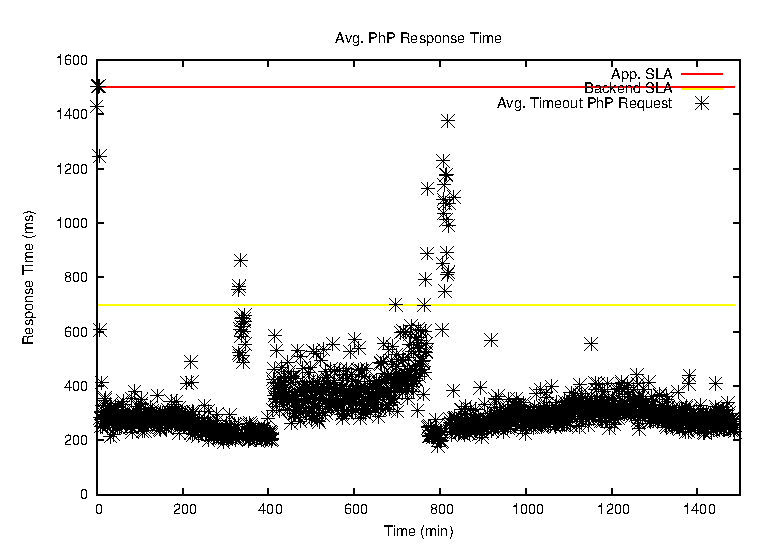
\includegraphics[width=0.49\textwidth, height=6cm]{./images/homogeneous/avgTimeout_PhP_naive}
\end{center}
\caption{PhP resp. time on DAS4 -- Load-based.}
\label{naiveDas4}
\end{figure}

\subsubsection{Resource consumption}

Nevertheless to better understand the behavior of both algorithms, we may also focus on the resource consumption illustrated on Figure~\ref{resComDas4}. Firstly, the excessive reactive behavior of the load-based algorithm is again illustrated at the interval \emph{t=350min} and \emph{t=820min}, where two scaling operations under-provision the system during a short period of time. These provisioning decisions provoked fluctuations in the system performance that incremented the financial cost, as well as throughput alterations under the same intervals of time, as depicted on Figure~\ref{naiveDas4}. When using the weighted-metrics feedback algorithm, the system makes provisioning decisions by analyzing workload's trend during a considerable interval of time. Scaling actions are only triggered when having constant alterations in the Wikipedia workload, providing a more efficient resource usage. Indeed, the workload alterations depicted on Figure~\ref{workload}, match with the provisioning decisions made by the weighted-metrics feedback algorithm on Figure~\ref{resComDas4}.

\begin{figure}
\begin{center}
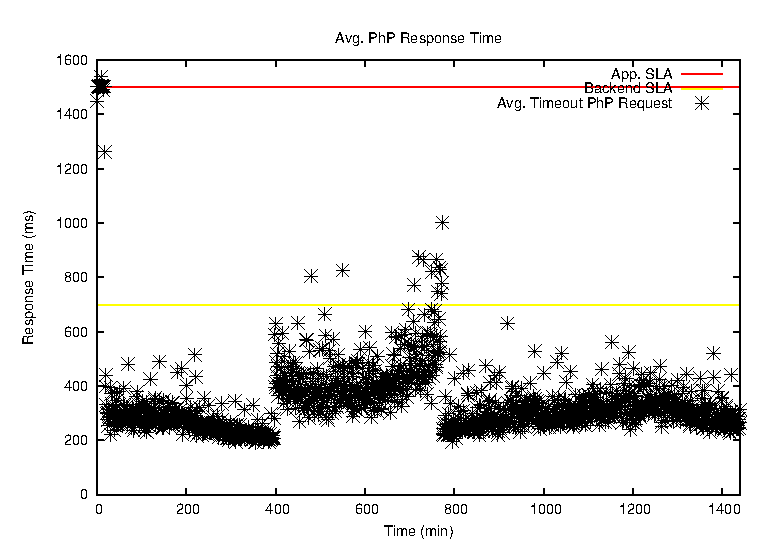
\includegraphics[width=0.49\textwidth, height=6cm]{./images/homogeneous/avgTimeout_PhP_history}
\end{center}
\caption{PhP resp. time on DAS4 -- Weighted-metrics feedback.}
\label{historyDas4}
\end{figure}

\begin{figure}
\begin{center}
\includegraphics[width=0.49\textwidth, height=5cm]{./images/homogeneous/numMachinesComp}
\end{center}
\caption{Resource consumption on DAS4.}
\label{resComDas4}
\end{figure}

\subsubsection{Discussion}

Using the load-based provisioning algorithm, the system performance fluctuates greatly following a pattern similar to the web traffic that increases the number of SLO violations. The reactive behavior of this algorithm triggers scaling actions that affect to the system performance instead of improving it, and as a consequence, it is also wasteful in terms of resource consumption. Unlike weighted-metrics feedback algorithm offers an efficient resource usage and a constant performance behavior while meeting the application's SLO. Therefore this algorithm finds the trade-off between accuracy and cost savings.

Both algorithms are best-effort regarding the SLO fulfillment, and thereby temporal alterations of the workload (with a short duration of 5min approx.) cannot be handled. The heterogeneity of the PhP-served pages containing images and requiring multiple Db queries, and the startup time of VMs, are in part responsible of these SLO violations. 

%It avoid to under-provisioning in two occasions  while decreases the number of SLA violation. However, the naive alg. is vulnerable to temporal bursty workload variations (10 min), an increment of SLA violated is caused by under-provisioning operations in conjunction with workload variations. 



\subsection{Heterogeneous Infrastructure}

Our experiments on EC2 used small instances for the PhP service (manager and agents) and  a medium instance for the MySQL service (agent). EC2 small instances provision VMs equipped with 1 EC2 CPU, and 1.7GiB of memory, while medium instances are equipped with 2 EC2 CPU's, and 3.75GiB of memory.

\subsubsection{SLO enforcement}

In the following, we analysis the behavior of our algorithms when making provisioning decisions on a heterogeneous infrastructure. Figure~\ref{naiveEC2}, Figure~\ref{historyEC2} and Figure~\ref{historyWeightEC2} show the system performance of the load-based, weighted-metrics feedback and profiling-based algorithms, respectively. As depicted on Figure~\ref{naiveEC2}, the performance fluctuates greatly following an irregular pattern when using the load-based algorithm. More precisely, two of the three workload peaks caused at \emph{t=300min} and \emph{t=820min}, are explained by looking at the variations on the Wikipedia workload described on Figure~\ref{workload}. However, there is a third peak between \emph{t=400min} and \emph{t=600min} that corresponds to the interval of time on which the workload trace experiences a significant drop in the request volumes. This explains the degradation of the SLO fulfillment as an effect associated to very frequent scaling actions. 

On the other hand, Figure~\ref{historyEC2} and Figure~\ref{historyWeightEC2} show as the weighted-metric feedback and profiling-based algorithm behave similarly. Even though both algorithms are best-effort, there is an important reduction in the number of SLO violations during the trace execution. In particular, the weighted-metric feedback algorithm reduces the SLO violations in a  41.3\%, while the profiling algorithm does it in a 47.6\%. Like on DAS-4, the weighted-metrics feedback algorithm follows a constant performance pattern without having sharp and sudden workload alterations. Besides, as shown on Figure~\ref{historyWeightEC2}, the profiling-based algorithm has a similar behavior to the weighed-metrics feedback algorithm in terms of system performance, however. The profiling-based algorithm improves the SLO enforcement in a 6.3\% in comparison with the feedback algorithm at the client's side. Therefore we demonstrate how the use of workload-mix and flexible load-balancing techniques, although intrusive, do not cause time delays or excessive throughput alterations. 



\begin{figure}
\begin{center}
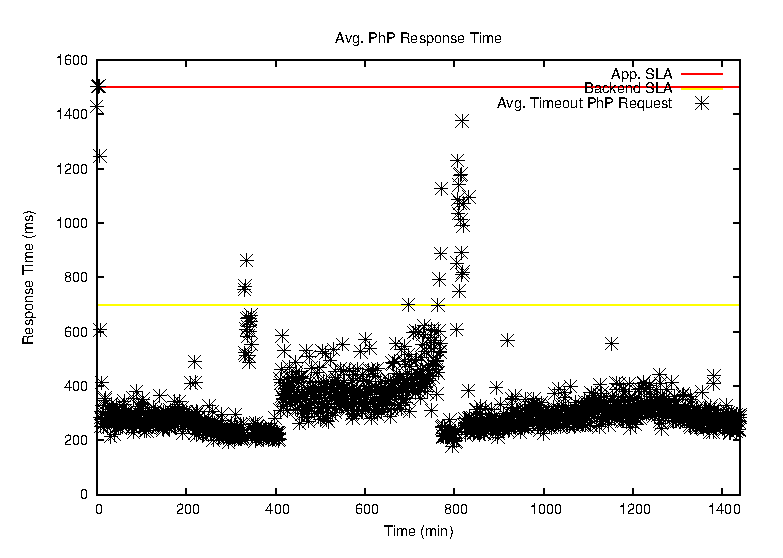
\includegraphics[width=0.49\textwidth, height=6cm]{./images/heterogeneous/avgTimeout_PhP_naive}
\end{center}
\caption{PhP  response time on EC2 -- Load-based.}
\label{naiveEC2}
\end{figure}


\begin{figure}
\begin{center}
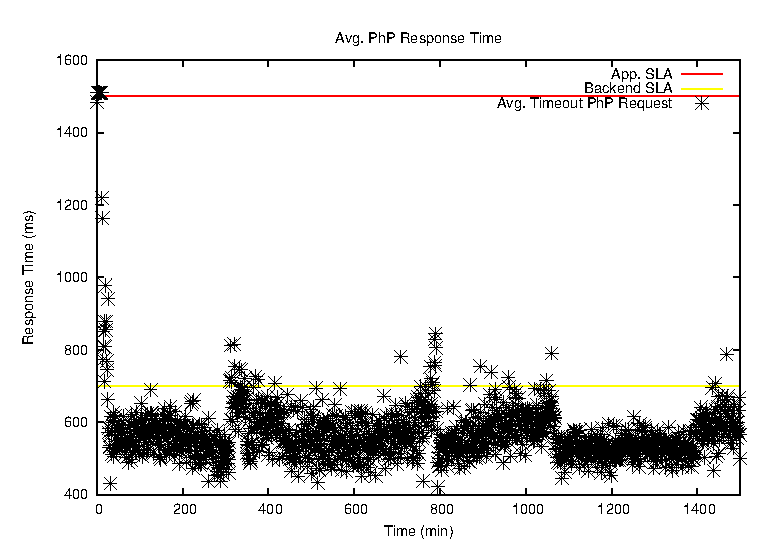
\includegraphics[width=0.49\textwidth, height=6cm]{./images/heterogeneous/avgTimeout_PhP_history}
\end{center}
\caption{PhP resp. time on EC2-- Weighed-metrics feedback.}
\label{historyEC2}
\end{figure}

\begin{figure}
\begin{center}
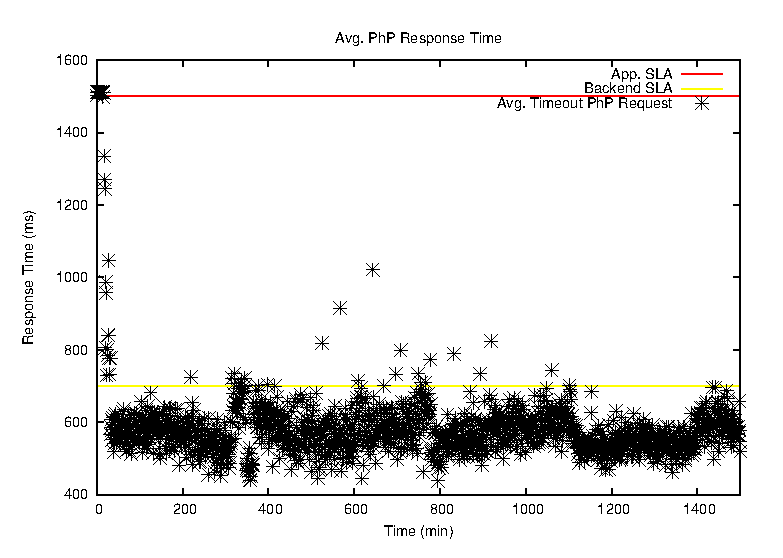
\includegraphics[width=0.49\textwidth, height=6cm]{./images/heterogeneous/avgTimeout_PhP_weightHistory}
\end{center}
\caption{ PhP resp. time on EC2-- Profiling-based.}
\label{historyWeightEC2}
\end{figure}

\subsubsection{Resource consumption}

The resource usage on EC2 presents important alterations as shown on Figure~\ref{resEC2}. When using the load-based provisioning, the fluctuations in the system performance are explained as a result of a high frequency of scaling operations. In concrete, these fluctuations caused at the interval of time comprised between \emph{t=400min} and \emph{t=500min} (see on Figure~\ref{naiveEC2}) match with the provisioning decisions made during the same interval of time on Figure~\ref{resEC2}. If we now pay attention to the weighted-metrics feedback, and profiling-based algorithms, their resource consumptions are identical along the execution. Indeed, both algorithms decided to scale out the system during the interval of time comprised between \emph{t=1050min} and \emph{t=1400min}, to prevent future SLO violations that occurred when using the load-based algorithm. In particular, this situation demonstrates the benefits of using flexible threshold ranges to provide a predictive provisioning mechanism, thus improving the user experience.


\begin{figure}
\begin{center}
\includegraphics[width=0.49\textwidth, height=5cm]{./images/heterogeneous/numMachinesCompEC2}
\end{center}
\caption{Resource consumption on EC2.}
\label{resEC2}
\end{figure}


\subsubsection{Discussion}


\fixme{Aggressive provisioning also increases the chances of degraded application performance due to the accompanying increase in violation of performance thresholds.}

\subsection{Discussion}



Generally, the result of our measurements show how the behavioral performance pattern and the resource consumption vary depending on the infrastructures on which we ran our experiments. Different hardware configurations such as those provided by DAS-4 and EC2, offer two distinct scenarios to validate our provisioning algorithms.  In these experiments, we demonstrate how trigger-based provisioning mechanisms can affect the system performance instead of improving it, as well as are wasteful in terms of resource usage. Workload-aware load-balancing technique, although intrusive, was included and used without producing performance alterations. In fact, this technique slightly reduced the number of SLO violations in comparison with the results obtained using weighted-metrics feedback algorithm. We also show the benefits by using weighted-metrics feedback and profiling-based provisioning algorithms which aims to find the trade-off between the accuracy and cost savings. 

%the flexible threshold ranges were pre-defined before execution for all VMs. These threshold values might be %changed depending the type of instance to be provisioned. Therefore, we believe that offline profiling techniques %may be used to define these values depending of the type of instance, thus improving the effectiveness of our %predictions.

%Today's resource provisioning systems define SLO's based on desirable threshold values for an application (CPU %$<$ 70\% and resp. time $<$= 700ms). However, these threshold values change depending the type of instance %to be provisioned (\emph{i.e.,} small instances 200 $<$ resp. time $<$ 500, while medium instances 200 $<$ %response time $<$ 600). In order to improve the accuracy of these algorithms, we consider that provisioning %decisions have to take into account two threshold ranges: (i) desirable threshold values for the whole application; %(ii) specific threshold values for each machine. Thus, to determine these machine-specific threshold values, offline %profiling techniques have to train during a period of time 



